	\lstset{float, emph={Scheduler, Job, Executor, Resource, DEMAND, RELEASE,
	PathDeclaration, ACCESS, PolicyDefinitions, JobReference, ResReference,
	builtin, new, Condition}, emphstyle=\textbf}
	
	
	\section{Flexible task scheduling with an automatically generated scheduler}
	\label{sec:taskScheduling}
	\label{sec:problem}
	One specific domain in which embedded controller software frequently performs
	optimisation is that of \emph{allocating resources to jobs over a period of time
	while optimising one or more objectives}~\cite{Brucker:book}.
	The component performing this optimisation is called \emph{scheduler}; it has a
	direct impact on resource management and, as a consequence, system performance.
	It is evident that a scheduler communicates with multiple system components,
	therefore its implementation is likely to be highly coupled.
	The design issues attached to a system scheduler can be categorised in two
	parts:
	% the connection between the initial, abstract definition of the "parts" was not
	% clear. also if you explain it immediately afterward, just give the explanation
	% and skip the "abstract definition"
	
	% \item The scheduler's internal characteristics and whether it satisfies the
	% scheduling requirements of a given system, and (2) others that are concerned
	% with the scheduler's integration to a base system.
	\begin{enumerate}
	\item \emph{Specification of scheduler components.} A scheduler component consists of (1) information about the base system in the
	form of data structures, (2) communication interfaces with the base system, and (3) a \emph{scheduling
	algorithm} that can solve the scheduling problem according to the objectives of that base system.
	The concrete definition of these elements may vary greatly depending on the
	application area: The scheduling requirements (on information, communication and objective) of a safety-critical system is
	very different from those of an operating system. The challenge lies in
	expressing system characteristics and the desired scheduling algorithm at the
	same level and defining the scheduling algorithm with the tasks and resources of
	the base system.
	
	\item \emph{Non-intrusive integration of schedulers.} Recalling the scheduling definition in the first paragraph, it is obvious that a
	scheduler has to constantly communicate about the current state of the
	resources and tasks, and at the same
	time must enforce constraints which might be predefined or introduced
	on-the-fly. These aspects alone pose a challenge in creating expressive and
	flexible interfaces for the scheduler. However there is another challenge which
	is the by-product of software/system evolution. Since schedulers involve system-specific parts, when systems evolve it is necessary to alter or -- depending on
	the amount of change performed in the system -- completely replace the scheduler.
	This is difficult given the scheduler's tight integration within the system
	software.
	This problem calls for a non-intrusive integration mechanism between the
	scheduler and the system and a cost-effective way of altering/replacing the
	scheduler implementation.
	\end{enumerate}
	
	\subsection{Scheduling workbench}
	\label{sect:approach}
	%\textbf{(CB: it would be nice to give this section another title since there
	%is already a section called approach. Maybe "Scheduling Workbench" (?))}
	
	We have developed a \emph{Scheduling Workbench}, to \emph{model and integrate
	schedulers into existing applications} (an overview is depicted in Figure \ref{fig:approach}).
	We have \emph{not} developed new scheduling algorithms, but provide a means to easily integrate schedulers into a system. Our ``domain-specific scheduling language'' acts as a meta-model and the entities involved in the scheduling process as well as the interface between them and a scheduling algorithm can be defined in this meta-model. Thus, ``generated scheduler'' refers to code which is generated from the ``scheduler specification'' and which interfaces with an implementation of a scheduling algorithm.
	
	The first step of development of such a workbench is a comprehensive domain
	analysis. Domain analysis is the process where the fundamental domain concepts
	and their variability is determined. In domain modelling these concepts and their
	relationships are expressed in a model. In Figure \ref{fig:approach} this model
	is shown as \emph{scheduling domain knowledge}. From this model we have derived
	a grammar for a scheduling domain-specific language, shown as an octagon
	in Figure \ref{fig:approach} connected to scheduling domain knowledge.
	
% 	\begin{figure}
% 	\begin{center}
% 	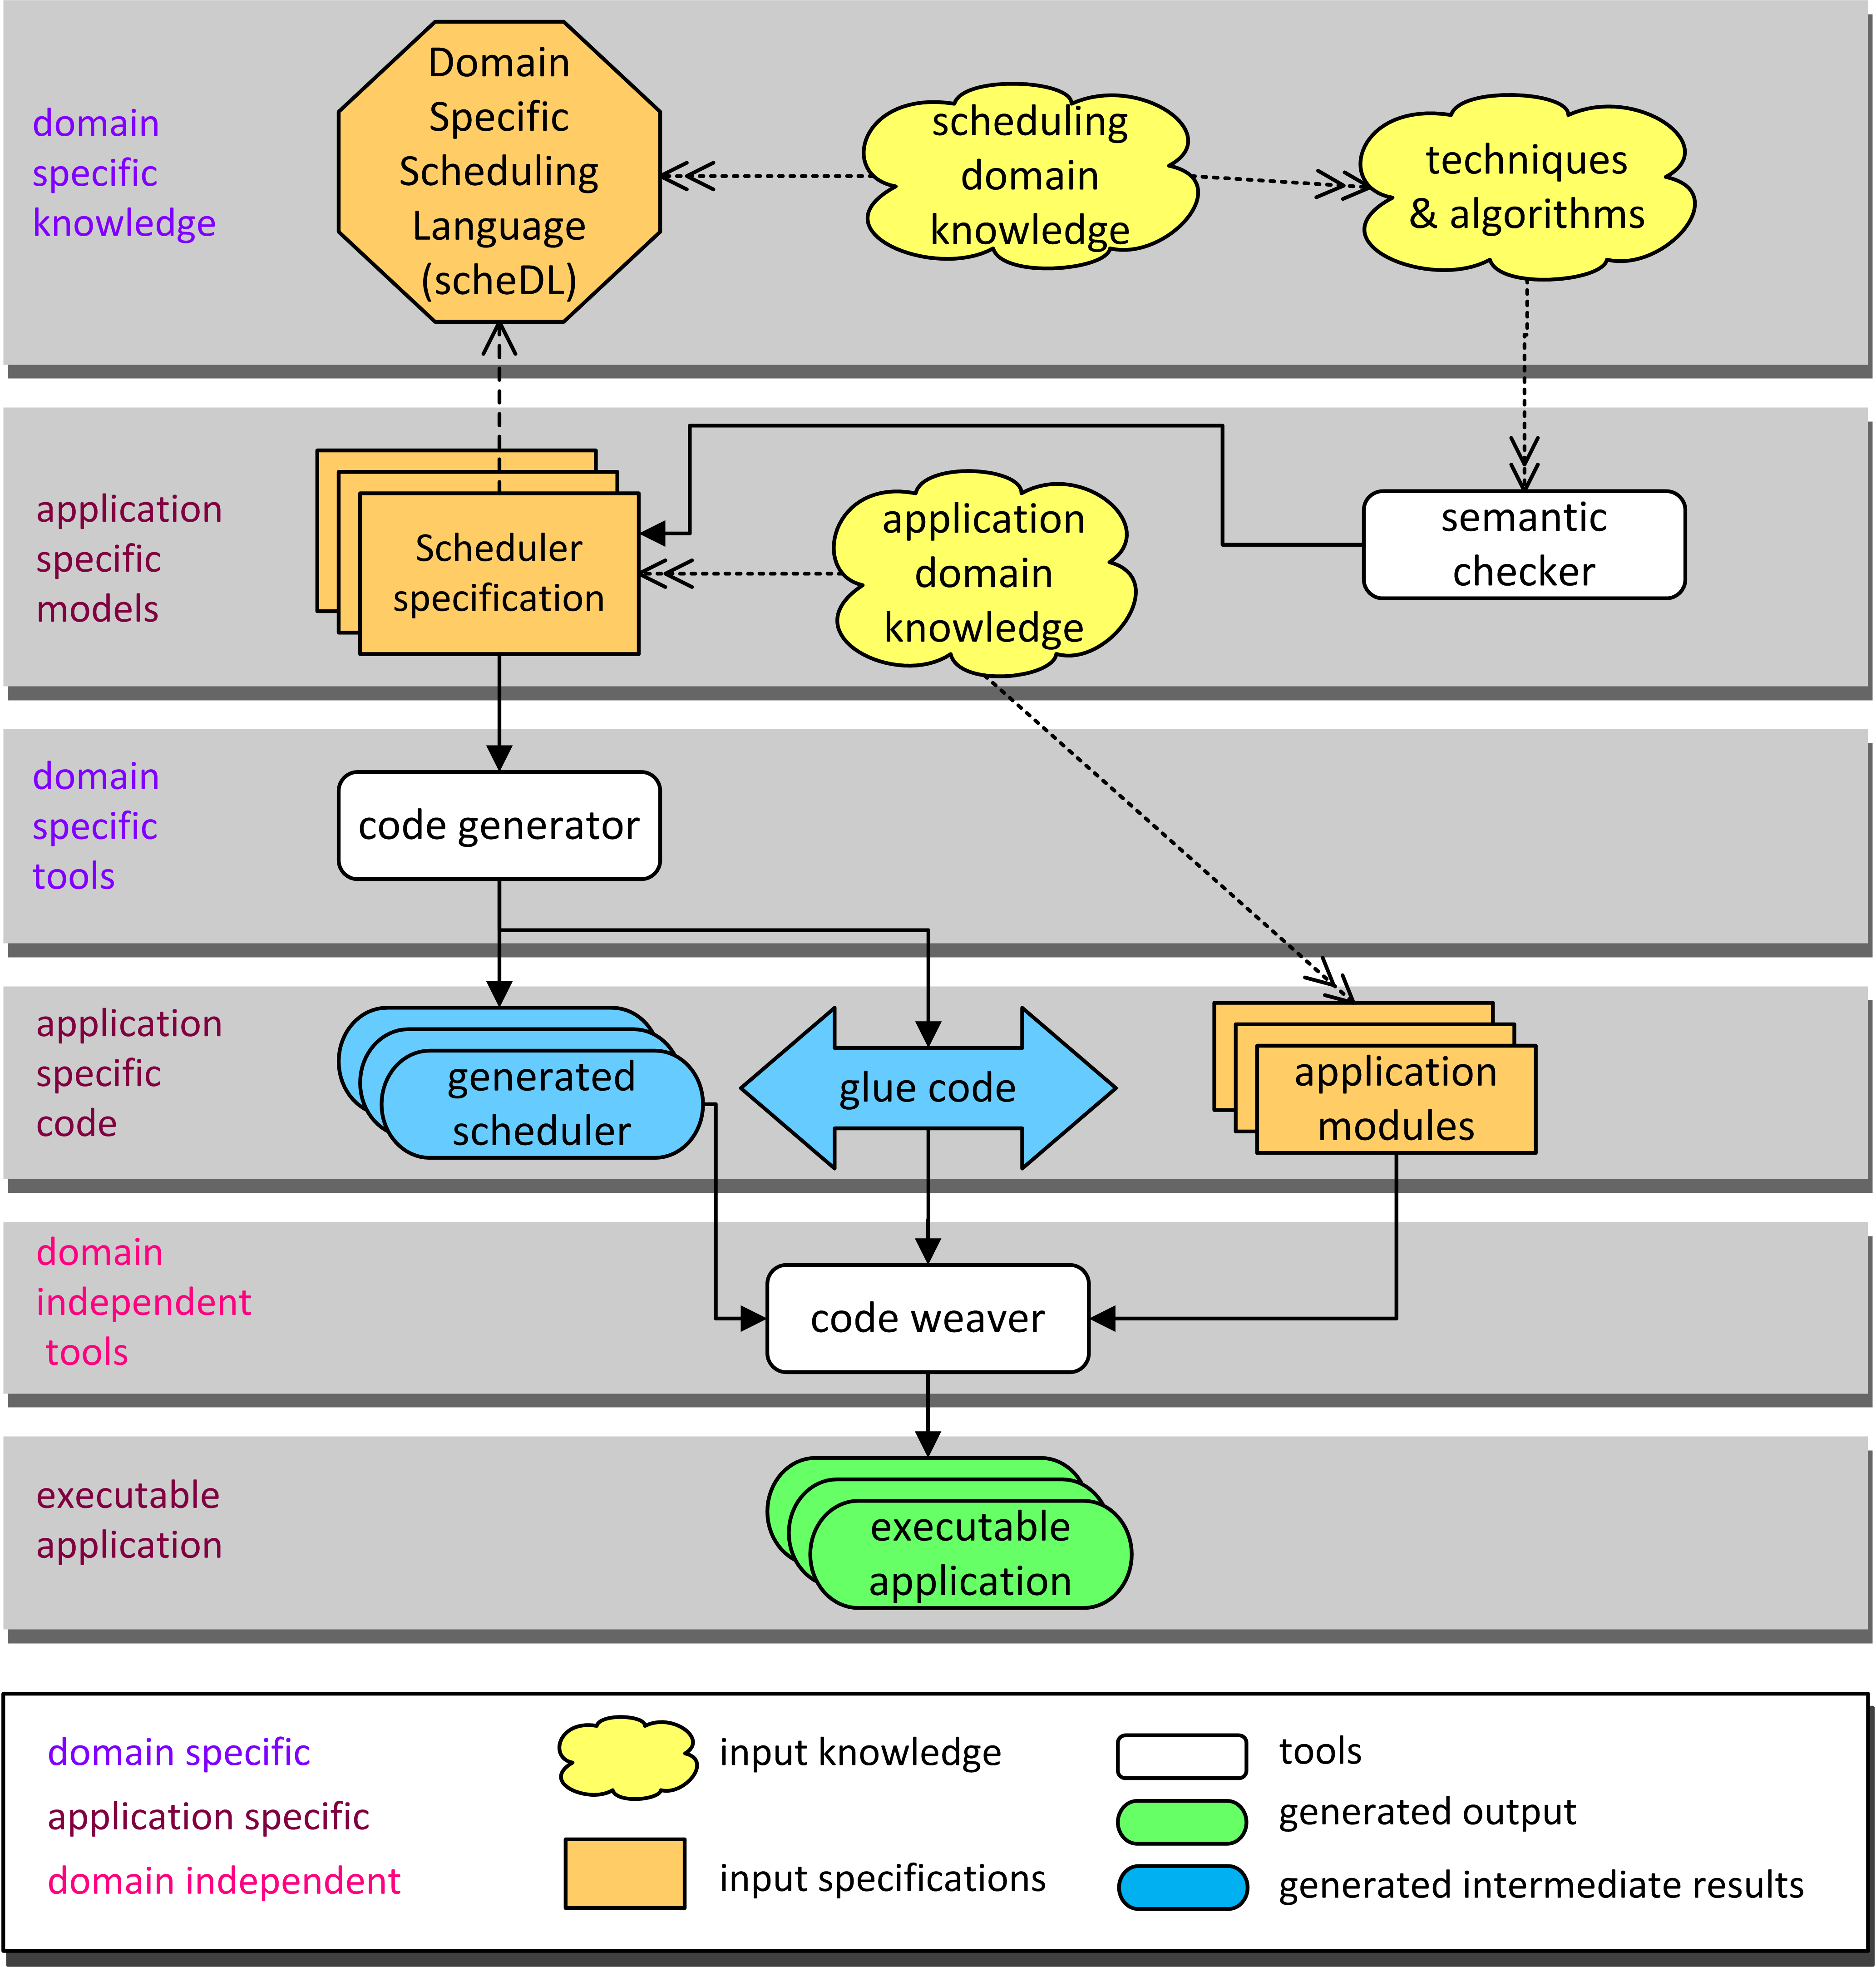
\includegraphics[width=\textwidth]{chapteroce/images/approach_new.png}
% 	\caption{Our approach instantiated for the scheduling domain.}
% 	\label{fig:approach}
% 	\end{center}
% 	\end{figure}
	
	\subsubsection{Domain analysis and modelling}
	% it's not the purpose to teach about domain analysis ... just say what you actually did
	% better write in active voice
	For domain analysis we have analysed commonalities and variabilities of scheduling approaches.
	We started by extracting the core domain concepts by means of a literature study
	and identifying the building blocks of the scheduling domain. After finding the
	core concepts, we have analysed the variations of these concepts.
	We have expressed our findings about the domain using feature modelling \cite{kang1990feature}. 
	
	In Figure \ref{fig:feature} a feature model for scheduling is shown
	(the full model can be found in \cite{Hatun:2011:FMD:1960518.1960520}).
	In the feature model notation every domain concept
	is mapped onto abstract features and their variations are mapped
	onto concrete features. For example, if we look at the \textbf{deadline} feature,
	we see that a deadline can be either \textbf{hard} or \textbf{soft}. It is also
	possible to define cross-tree constraints as logical expressions, shown in
	Figure \ref{fig:feature} below the feature tree. This is additional semantic
	information about the domain which is used to implement the \emph{semantic
	checker} shown in Figure \ref{fig:approach}.
	
	\begin{center}
	\begin{figure}
	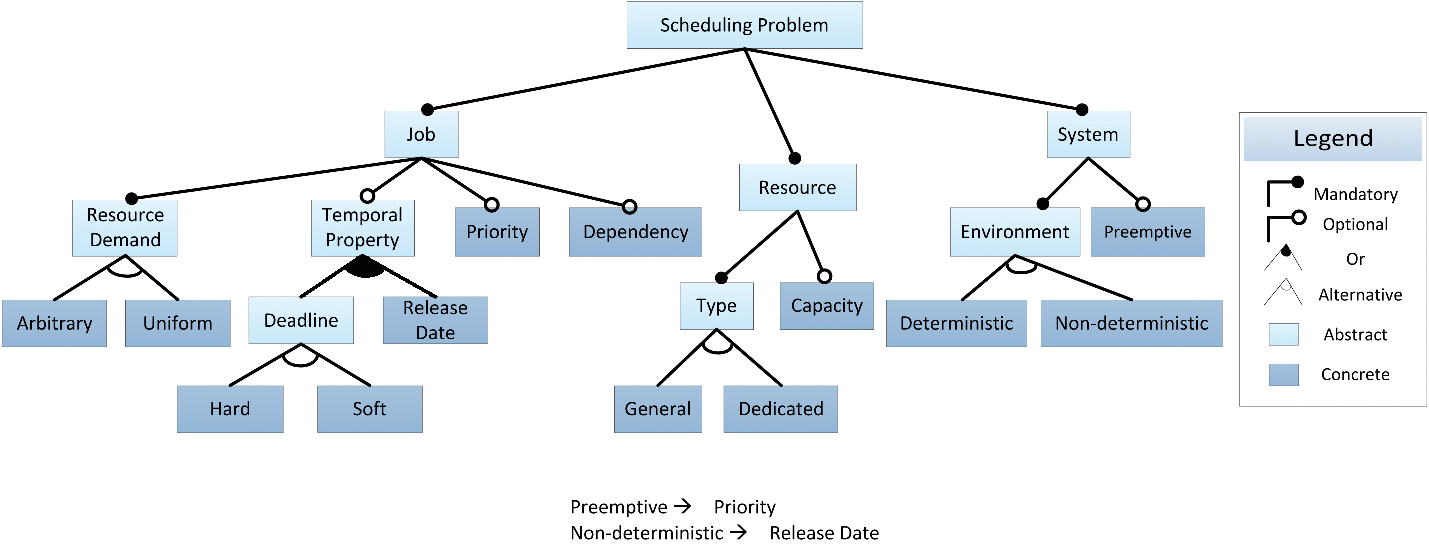
\includegraphics[width=\textwidth]{chapteroce/images/features.pdf}
	\caption{A simplified version of the feature model for scheduling.}
	\label{fig:feature}
	\end{figure}
	\end{center}
	%
	\subsubsection{Domain-specific language design and code generation}
	%the feature model corresponds to the abstract syntax, or to a meta-model of valid abstract syntax trees
	%but it is not the AST which is a concrete tree for one program.
	%use spell checker
	%you do not "populate" a grammar or an AST with keywords. What are other "structural elements"?
	%Mernik did not publish the paper, but ACM or Springer did
	%no abbreviations "doesn't"
	Following the advice of Mernik et al. \cite{Mernik2005}, we have designed a DSL for the scheduling domain (the ``scheduling domain-specific language'', \textsf{scheDL}) using the feature 
	model presented in the previous subsection. We have used the feature model as
	the abstract syntax and turned it into the concrete grammar of our \textsf{scheDL} language, especially by defining keywords.
	%Why say this below? Your DSL can be executed ...
	%A DSL does not have to be executable to be useful.
	%It can just be used to
	%communicate requirements concerning a particular domain.
	In our approach we chose to generate \emph{general-purpose language (GPL)} code from our DSL, which is called
	generative programming \cite{Czarnecki:overview}.
	%If you write (e.g. Java, C++) the e.g. already shows that you just give an example, thus nothing like ... or etc. is needed
	This method allows a user to
	program on a higher abstraction layer, and to obtain code in widely supported and robust programming languages (e.g. Java, or C++) at the same time. The \emph{code generator} knows how to process a \emph{scheduler specification} and
	how to incorporate it with \emph{application domain knowledge} to obtain GPL code (cf. the arrow from ``application domain knowledge'' to `` code generator'' in Figure~\ref{fig:approach}).
	
	%the *benefits* do not "handle" anything
	Let us illustrate the benefits of our approach by explaining how we handle the
	two main challenges presented in Section \ref{sec:problem}.
	The first one expresses the requirements of a scheduling problem
	using the concepts found in the scheduling domain. At the end of the domain
	analysis and modelling phase, we have a model of the scheduling domain, which
	includes core concepts, their variations and the relationships of those concepts.  From this
	model we have created a grammar for \textsf{scheDL}. Using this language we can define \textsf{job}s,
	\textsf{resource}s and \textsf{scheduler}s with concise domain specific language
	constructs.
	
	The block structure syntax of \textsf{scheDL} promotes readability and
	makes it accessible even to non-programmers. Using a DSL we are able to describe
	the scheduling requirements and a scheduler concisely. This is also useful for
	maintainability since altering the scheduler only requires changing the short specification file written in \textsf{scheDL}.
	
	The second challenge mentioned in Section \ref{sec:problem} concerns a
	scheduler's tight integration with a system. In \textsf{scheDL} we offer
	language constructs to model behavioural interactions between the system and the
	scheduler in the form of event declarations. During code generation these event
	declarations are turned into software components of a special kind, called
	\emph{aspects}. The language mechanism of aspects enables to compose the
	behaviour of aspect components with the events of other components without
	intrusively modifying them to make the events explicit in the code.
	
	\subsection{Example cases}
	% if a sentence starts with the same subject as the previous sentence ended,
	% probably the sentences can be combined
	We have tested our Scheduling Workbench on the \texttt{DemoPrinter} application,
	which has been developed in Java and simulates a professional printer. Figure \ref{fig:demoprinter}
	shows the static structure of this application; for brevity we have left out
	some utility classes from this view.
	In the following, we demonstrate out workbench by applying to to three example cases. The examples are written in
	\textsf{scheDL}\footnote{In listings, \textsf{scheDL} language keywords are
	shown in bold.}; the examples are \begin{inparaenum}[\itshape a\upshape)] \item
	replacing the existing scheduler of the demo printer, \item adding a new
	hardware component to be scheduled, and \item supporting multiple scheduling
	policies with the new scheduler\end{inparaenum}.
	\begin{figure}
	\begin{center}
	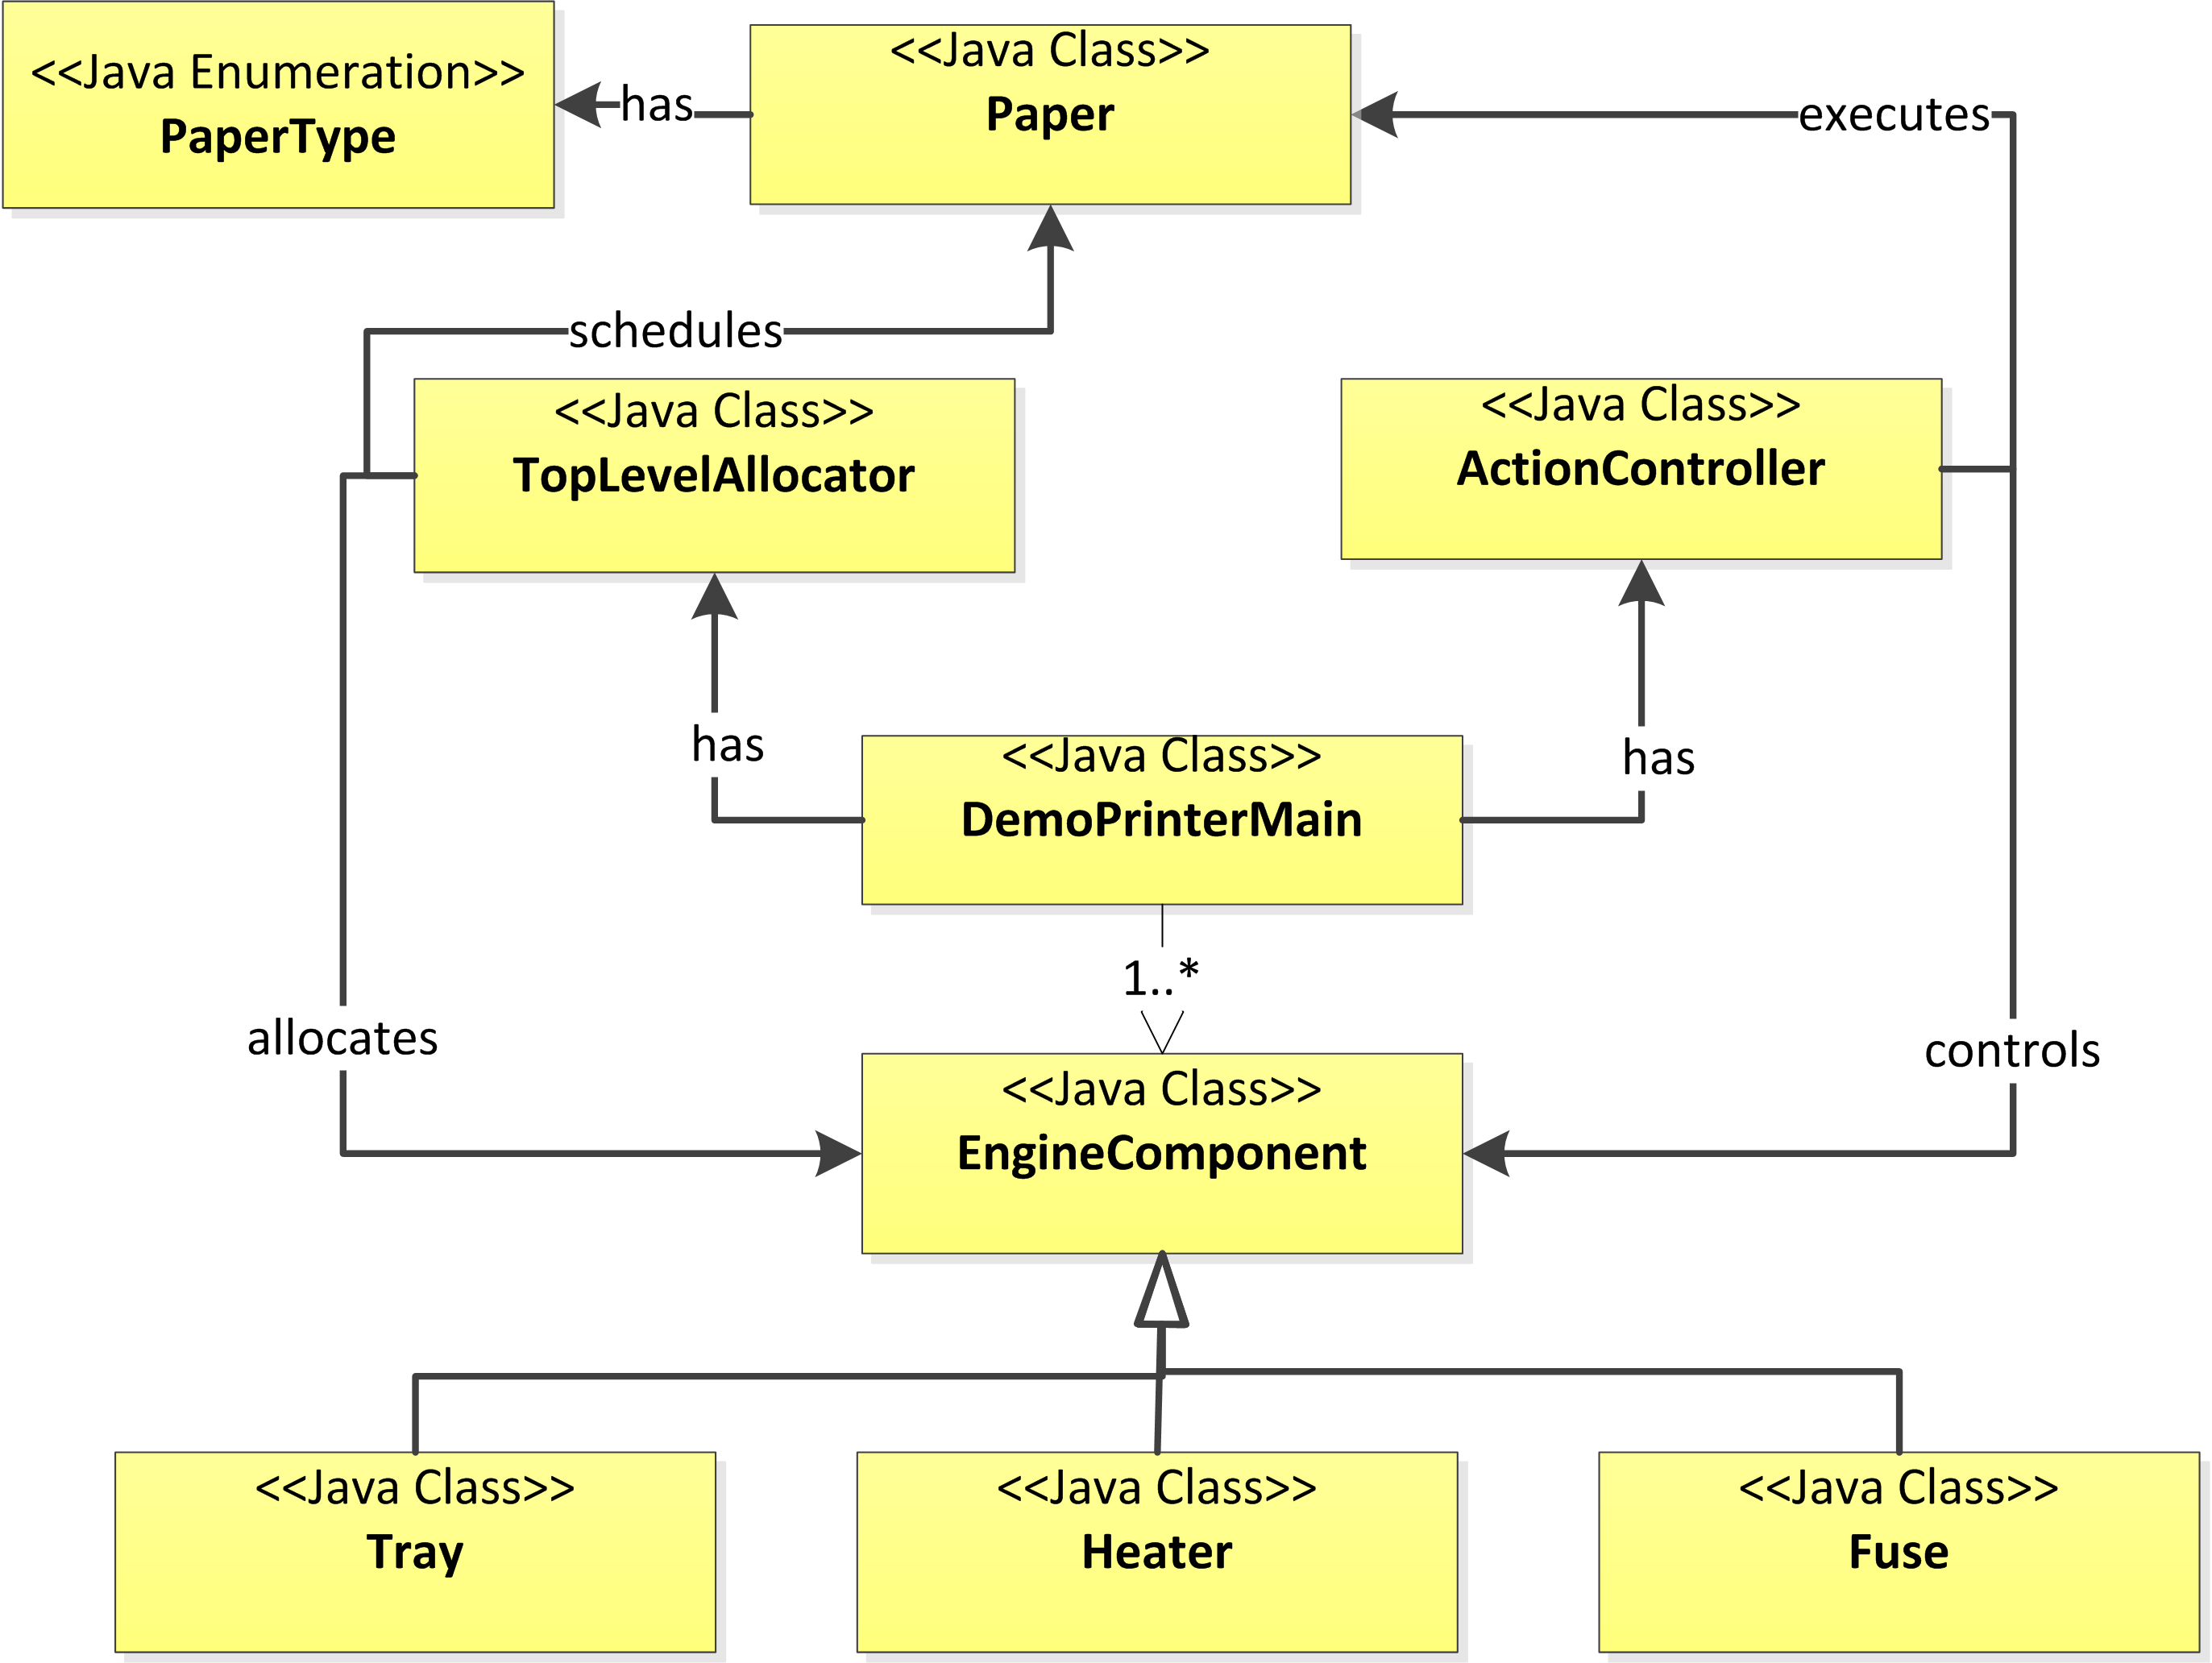
\includegraphics[width=0.75\textwidth]{chapteroce/images/demoprinter.png}
	\caption{The static structure of \texttt{DemoPrinter}.}
	\label{fig:demoprinter}
	\end{center}
	\end{figure}
	%
	\subsubsection{Replacing the scheduler in legacy code}
	%
	%use consistent naming (test case/example)
	In this example case, we replace the scheduler of the \texttt{DemoPrinter}
	using the Scheduling Workbench. The first step is to write a \textsf{scheDL} specification
	describing the kind of jobs and resources exist in the system. We also
	define a scheduler in the specification. In Listing \ref{lst:job} the definition
	of a \texttt{\textbf{Job}} is shown. A \texttt{\textbf{Job}} with the name \texttt{Paper} is
	defined. This job has an integer, the so-called release date, which is defined
	as the time a job becomes available. It is also possible to define properties like deadline, or
	priority. In the definition we also reference \texttt{\textbf{Executor}}
	resources as a \texttt{\textbf{DEMAND}}, which means: In order to be able to execute a \texttt{Paper} job, we
	need a \texttt{Tray}, a \texttt{Heater} and a \texttt{Fuse}. The \texttt{newpath} property is a \emph{path
	declaration} which defines an order between the demanded resources. The scheduler has to consider processing times of the involved component such that paper jams are avoided and it can be ensured that components are ready when the paper arrives.
	%
\begin{lstlisting}[caption={Job definition.}, label={lst:job}]
Job Paper{
	RELEASE release_date Integer
	DEMAND Tray
	DEMAND Heater
	DEMAND Fuse
	newpath
}

PathDeclaration newpath{ Tray->Heater->Fuse }
\end{lstlisting}

	In Listing \ref{lst:exe} the definition of an Executor is shown. Every structure
	defined in \textsf{scheDL} must have unique name. Here we
	have defined the executor \texttt{Tray} as an executing resource with single
	access, which means it can only execute one job at a time. The same definition
	is made for \texttt{Heater} and \texttt{Fuse}.
	
\begin{lstlisting}[caption={Executor definition.}, label={lst:exe}] 
Executor Tray { 
	ACCESS single 
}
\end{lstlisting}
	%  \textbf{(CB: more consistent use of fonts for code. Make clear when you use
	% keywords in the text.)}
	The next step is to define the scheduler which will include references to the
	structures defined before. \texttt{\textbf{Scheduler}} is the central structure
	in \textsf{scheDL}; this is, only the structures referenced by the scheduler
	will be generated. Therefore, it is possible to define multiple jobs or
	resources in the same file even if they are not used. In Listing
	\ref{lst:scheduler} the scheduler definition for our example is shown. This
	scheduler definition basically describes a scheduler which assigns the three resources to sheets applying the \emph{First-Come First-Serve} policy.
	
\begin{lstlisting}[caption={Scheduler definition.}, label={lst:scheduler}]
Scheduler Myscheduler{ 
	PolicyDefinitions{ 
		builtin FCFS 
	} 
	JobReference{
		Paper 
	}
	ResReference{ 
		Tray 
		Heater 
		Fuse 
	} 
}
\end{lstlisting}
	%  it is the first time you talk about replacing. until here it was just about
	% defining a scheduler "replacement" is discussed below
	This is all the code needed for defining a scheduler for the
	\texttt{DemoPrinter} example. The jobs and resources are automatically mapped to
	classes with the same name in the \texttt{DemoPrinter} application.
	Figure \ref{fig:generated} illustrates this mapping for the engine components of
	the printer. Printer classes are extended by generated interfaces, but this
	relationship is encapsulated in aspects (the implementation layer shown in the
	figure).
	This way we can add behaviour to the \texttt{DemoPrinter} without altering its
	implementation.
	
	Given a \textsf{scheDL} specification, the Scheduling Workbench outputs code consisting
	of the user defined components, the scheduler and its helper classes, a library of scheduling
	policies declared in the \textsf{scheDL} specification, and
	abstract classes that capture domain concepts like job, resource, etc.
	%
	\begin{figure}
	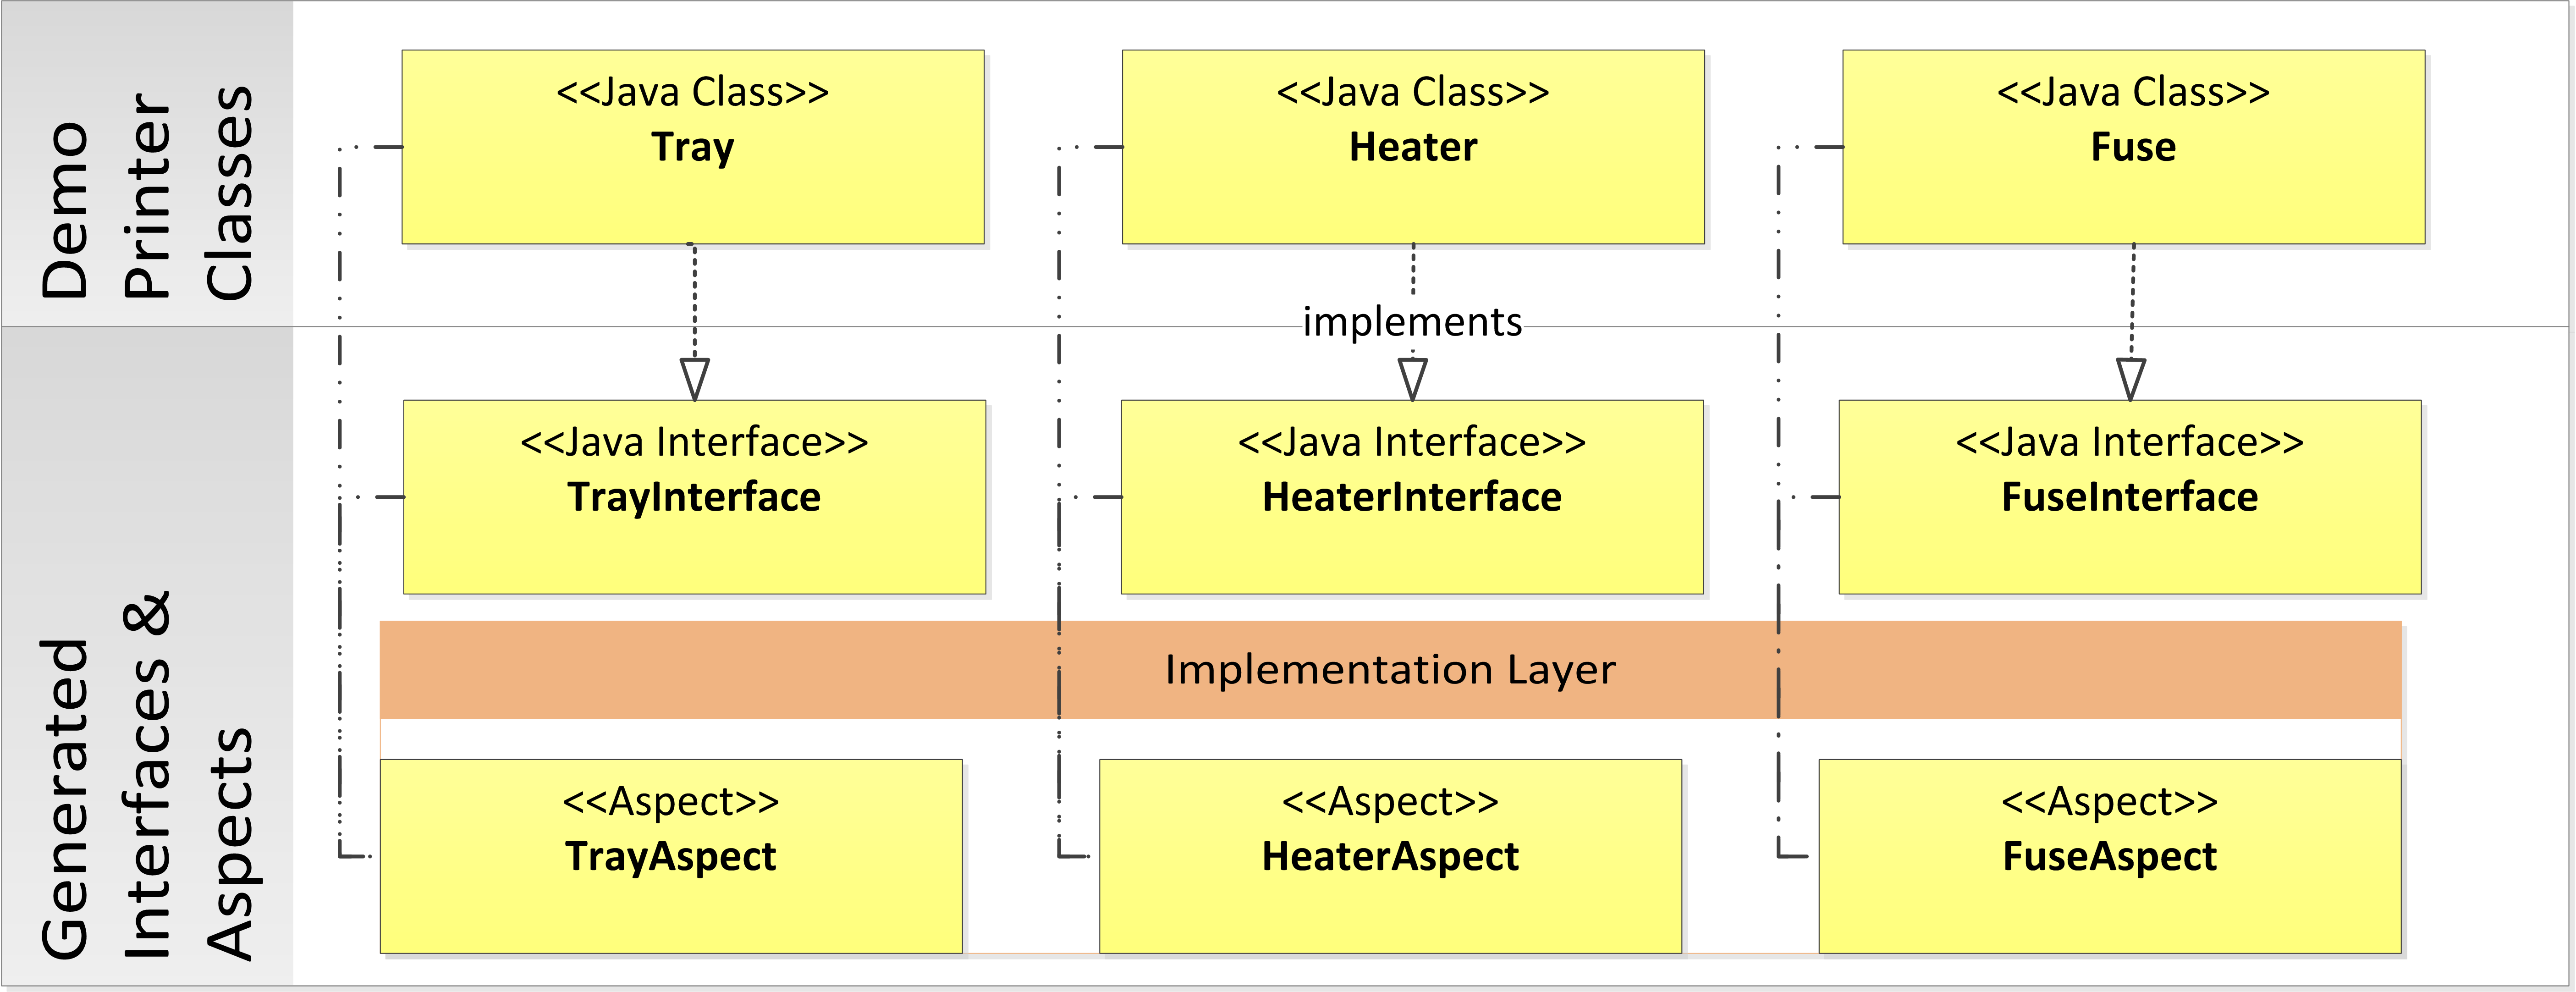
\includegraphics[width=\textwidth]{chapteroce/images/generated.png}
	\caption{Mapping of system classes and generated interfaces}
	\label{fig:generated}
	\end{figure}
	%
	Since the \texttt{DemoPrinter} application already contains a scheduler, the user has to find and disable its code after the generated code is imported, e.g., by removing the
	\texttt{TopLevelAllocator} class in the example. Then the new scheduler can be added to the
	base system, ready to work. A concise and fixed interface is provided with the
	scheduler to make it intuitive to use in the base system. The system's state
	after making this change can be seen in Figure \ref{fig:finalview}.
	If a scheduler in an application is developed in the Scheduling Workbench in the first place, switching the scheduler becomes even easier: Only the \textsf{scheDL} specification has to be replaced.
		
	%FIXME  layout of the listing has been lost?
	\subsubsection{Adding a component}
	In the second example we will illustrate what happens if a new component, namely a
	\texttt{Finisher}, is added to the system. In order to modify our scheduler
	software we only need to add a few lines of code to our \textsf{scheDL}
	specification. The applied changes are shown in Listing \ref{lst:addcomp}.
\begin{lstlisting}[caption={Extra code for adding a component.},label={lst:addcomp}]
Scheduler Myscheduler{
Job Paper{ 
	...
	DEMAND Finisher 
} 
Executor Finisher{ 
	ACCESS single 
} 
PathDeclaration newpath{ 
	Tray->Heater->Fuse->Finisher 
} 
Scheduler Myscheduler{ ...
	ResReference{ ...
		Finisher 
	} 
}
\end{lstlisting}
	We only had to add 5 lines to our \textsf{scheDL} specification to
	make sure 
	%\textbf{(CB: the sentence is incomplete. "that a new class" (is) what?)} 
	that a new class for \texttt{Finisher} and the necessary dependencies
	are generated connecting this class to the scheduler. After altering the
	specification the scheduler code needs to be regenerated and imported into the system code.
	Then the system is able to use the new component. The system's state after
	making this change can be seen in Figure \ref{fig:finalview}.
	
	\subsubsection{Supporting multiple policies}
	In the last example case, we add support to \texttt{MyScheduler} for supporting
	multiple policies. This means, the base system can switch policies when a
	condition changes, for example if the power is low it may choose a power-aware
	policy. This is important since it enhances system adaptivity greatly. In
	Listing \ref{lst:multiple} we show what must be added to our \textsf{scheDL} specification
	to support multiple policies. Firstly we define a resource called
	\texttt{Power} with limited capacity.
	%
\begin{lstlisting}[caption={Extra code for supporting multiple policies.},label={lst:multiple}] 
Resource Power{
	CAPACITY limited
}
Scheduler Myscheduler{
	PolicyDefinitions{
		builtin FCFS
		new UserPolicy
		Condition Policychange{
			resource: Power
			FCFS = "Power.getCapacity() >= 100";
			Userpolicy = "Power.getCapacity() < 100";
		}
	}
	...
}
\end{lstlisting}
	%
	Secondly, in the PolicyDefinitions block we declare two policies, one is First-Come
	First-Serve, provided by Scheduling Workbench's policy library, hence we
	distinguish it with the keyword \texttt{builtin}. The second one is a \emph{new}
	policy, meaning it will be implemented/provided by the user. If more than one
	scheduling policy is declared then a \emph{condition} for policy change needs to
	be defined (Benefit 2).
	
	We can define a condition in \textsf{scheDL} with the 
	\texttt{Condition} keyword, then referencing the structure triggering the policy change we define when each
	policy is valid. According to the condition defined in Listing
	\ref{lst:multiple} FCFS policy will be applied when the available power is more than or equal to 100, and UserPolicy will be applied
	when available power is less than 100. Figure \ref{fig:finalview} illustrates the system after applying this change.
	
	\subsection{Conclusion}
	
		In these example cases we have demonstrated how to create a scheduler
		with \textsf{scheDL}. We have also discussed the possibility to use custom scheduling policies allowing the user to customise
		certain aspects of their specification offering enhanced expressiveness.	
		The complete list of benefits provided by Scheduling Workbench are: 
		
		\begin{enumerate}[{Benefit} 1]
		  \item Domain concerns can be expressed intuitively from a higher level of
		  abstraction.
		  \item Complex domain constraints can be defined and checked; modelling
		  errors are reduced.
		  \item Software maintainability is increased through concise and understandable
		  DSL code.
		  \item Software evolution is eased by the underlying rich domain model.
		  \item Integrated editor and IDE support make programming in DSLs easy.
		  \item Code generation highly reduces manual labour spent on customising
		  general-purpose tools.
		  \item Easy system integration of generated code is provided through
		  non-invasive software engineering techniques.
		\end{enumerate}
		

				
	\begin{center}
	\begin{figure}
	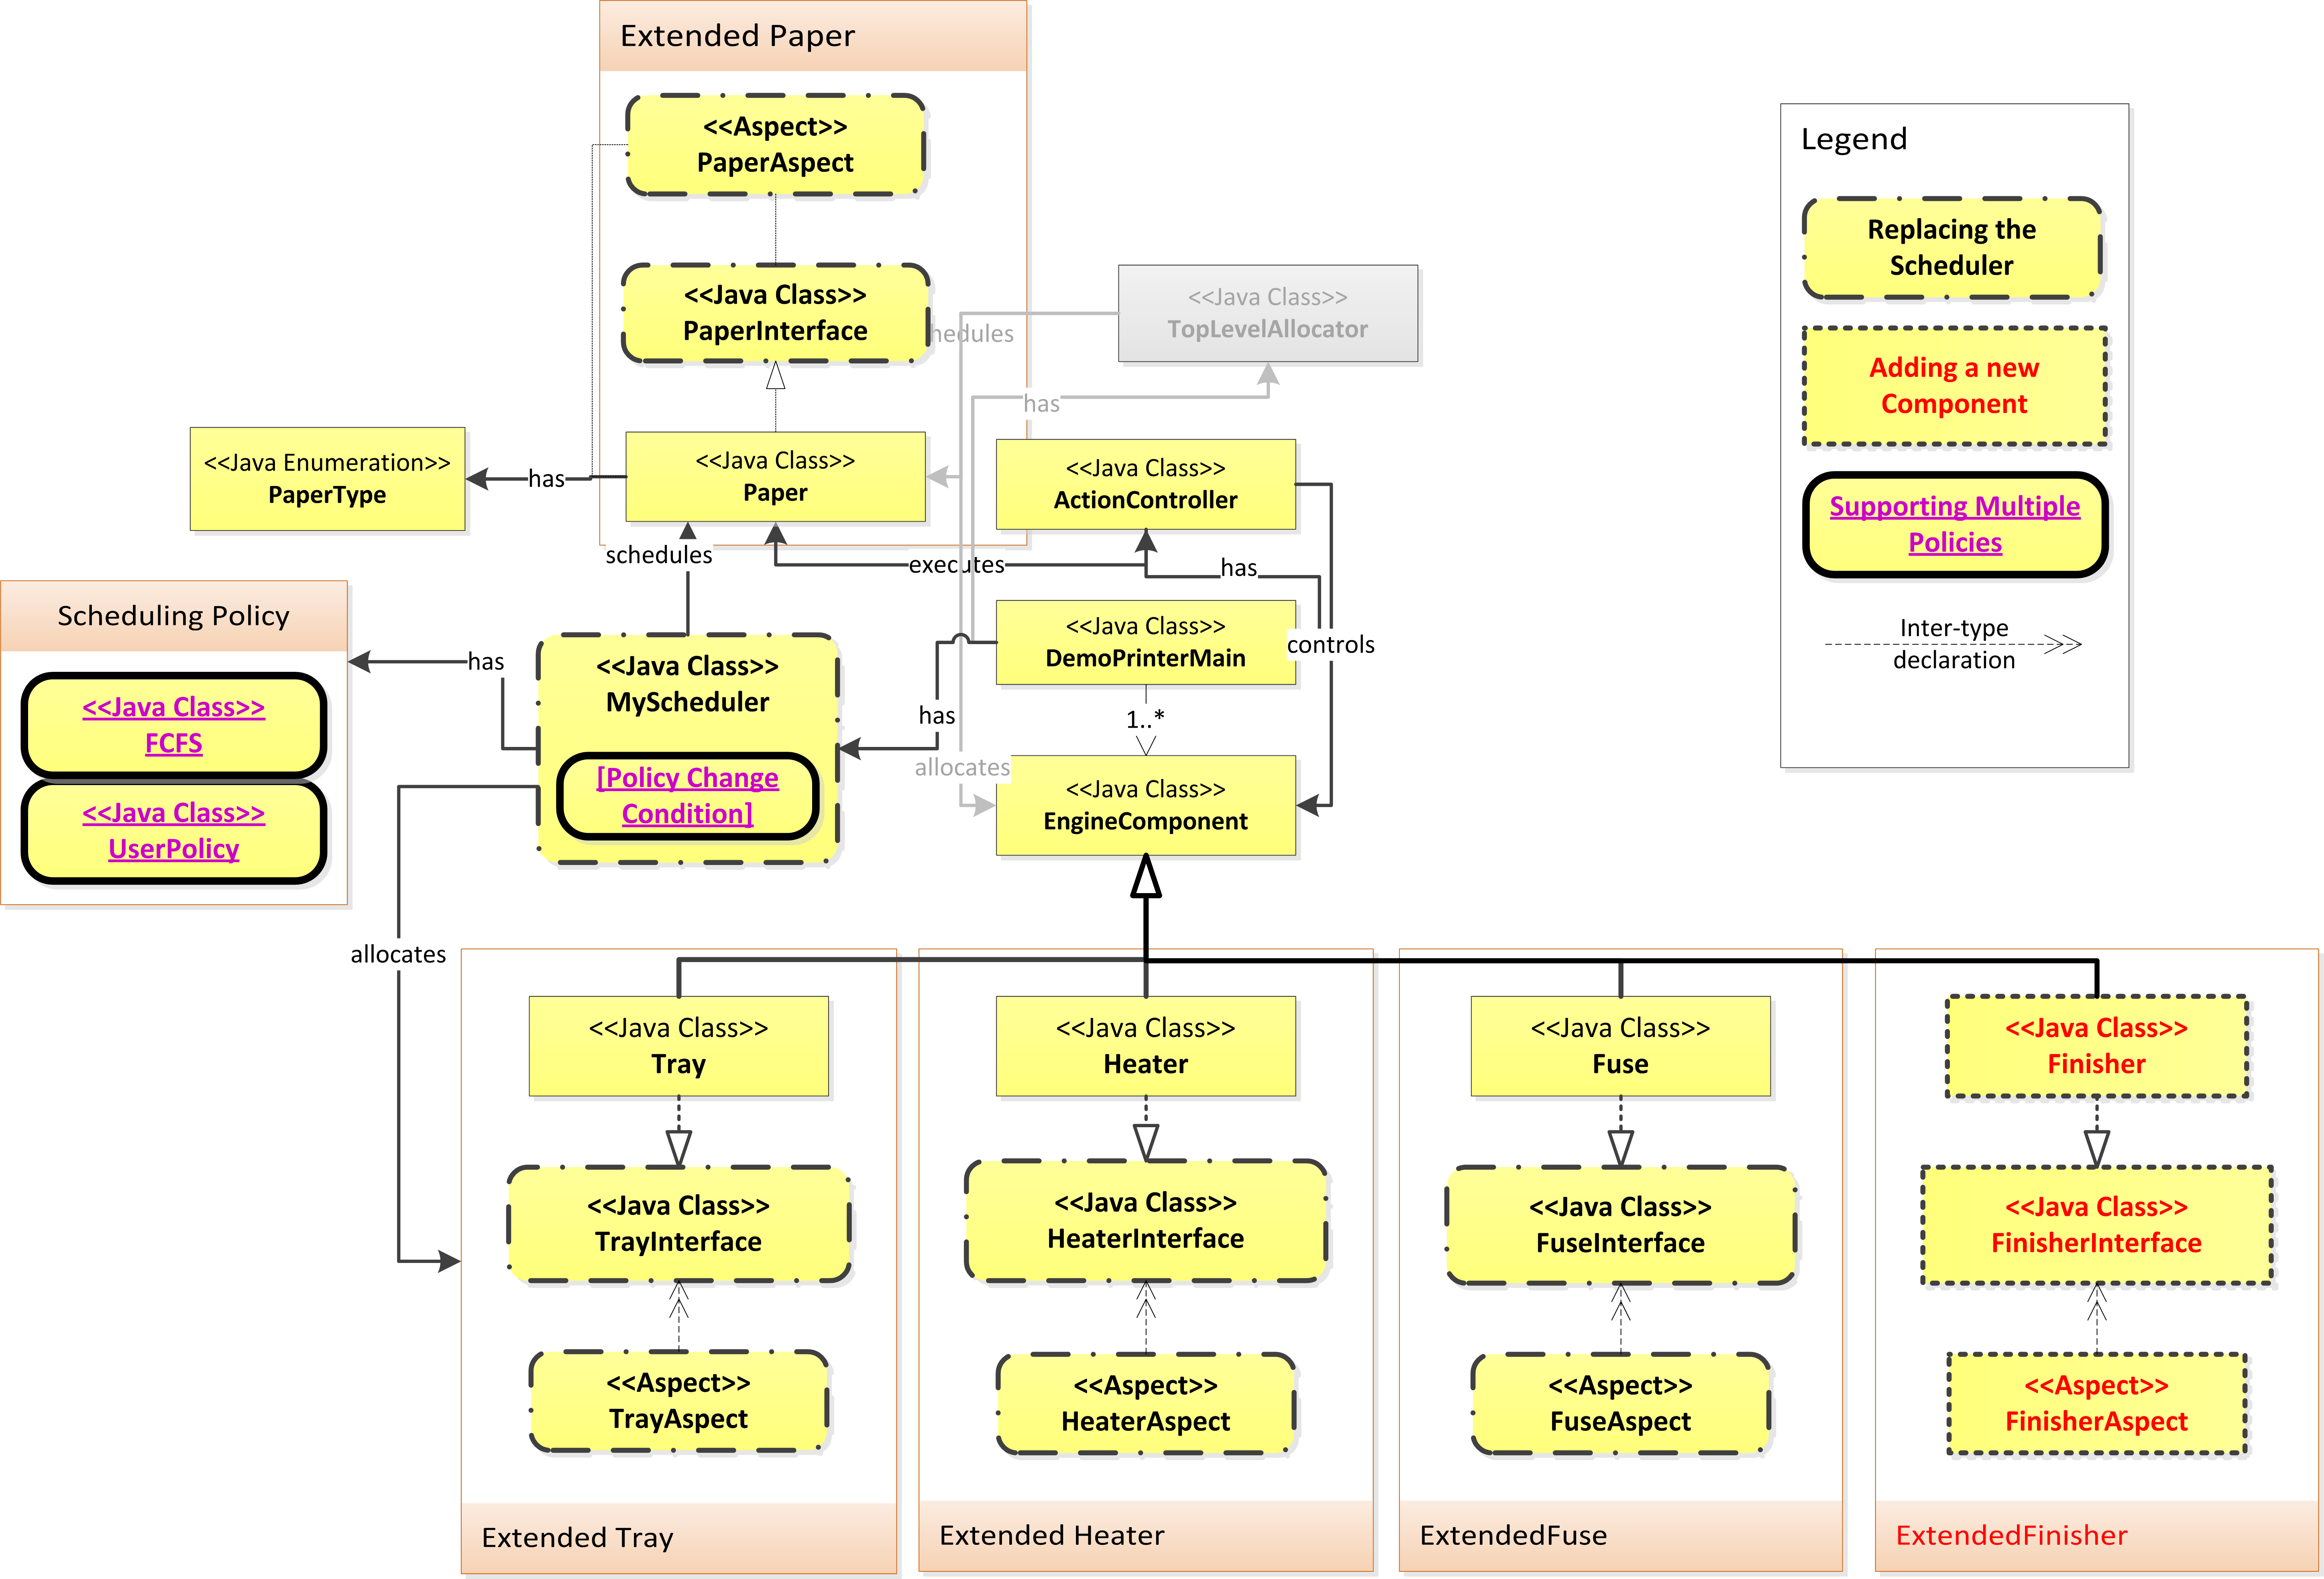
\includegraphics[height=\textwidth , angle=90]{chapteroce/images/finalview.png}
	\caption{The final view of the system after all example case.}
	\label{fig:finalview}
	\end{figure}
	\end{center}
	
